\section{Solving Burger’s Equation using Fourier Collocation}
The Fourier Collocation method was implemented using odd-numbered grid points defined as:
\begin{equation}
	x_j = \frac{2\pi}{N+1}j, \quad j \in [0, N]
\end{equation}
The Spatial derivatives were computed using the Fourier differentiation matrix $\tilde{D}$, and time integration was performed using th e 4th-order Runge-Kutta scheme.
\begin{equation}
	\begin{align}
		u_1     & = u^n + \frac{\Delta t}{2}F(u^n)                                             \\
		u_2     & = u^n + \frac{\Delta t}{2}F(u_1)                                             \\
		u_3     & = u^n + \Delta t F(u_2)                                                      \\
		u^{n+1} & = \frac{1}{3}\left[-u^n + u_1 + 2u_2 + u_3 + \frac{\Delta t}{2}F(u_3)\right]
	\end{align}
	\label{eq:}
\end{equation}
where $F(u^n) = -u^n\frac{\partial u^n}{\partial x} + \nu\frac{\partial^2 u^n}{\partial x^2}$.\newline
The time step was determined according to the following CFL condition
\begin{equation}
	\Delta t \leq \text{CFL} \times \left[\max_{x_j} \left(\frac{|u(x_j)|}{\Delta x} + \frac{\nu}{(\Delta x)^2}\right) \right]^{-1}
\end{equation}
\subsection{Determining Maximum CFL Values}
The maximum stable CFL values were determined experimentally for various grid sizes using a binary search method that tested different CFL values for each grid sizes.
\begin{enumerate}
	\item For each grid size $N$, we established an initial search interval $[\text{CFL}_{\text{low}}, \text{CFL}_{\text{high}}]$ with $\text{CFL}_{\text{low}} = 0.01$ and $\text{CFL}_{\text{high}} = 0.75$.
	\item We then used binary search to find the maximum stable CFL:
	      \begin{enumerate}
		      \item Set $\text{CFL}_{\text{test}} = (\text{CFL}_{\text{low}} + \text{CFL}_{\text{high}}) / 2$
		      \item Run the solver for a short time period (specifically $t = \pi/8$) using $\text{CFL}_{\text{test}}$
		      \item Check both the stability and accuracy of the solution:
		            \begin{itemize}
			            \item If the solution was stable (no NaN or Inf values) and accurate (error below a threshold of 0.1), set $\text{CFL}_{\text{low}} = \text{CFL}_{\text{test}}$
			            \item Otherwise, set $\text{CFL}_{\text{high}} = \text{CFL}_{\text{test}}$
		            \end{itemize}
		      \item Repeat until $\text{CFL}_{\text{high}} - \text{CFL}_{\text{low}} < \text{CFL}_{\text{tolerance}}$ (where $\text{CFL}_{\text{tolerance}} = 0.01$)
	      \end{enumerate}
\end{enumerate}
This ensures that CFL maintains stability and provides sufficient accuracy.
\begin{table}[H]
	\centering
	\begin{tabular}{|c|c|c|}
		\hline
		$N$ & Max CFL & Error at Max CFL \\
		\hline
		16  & 0.0100  & 0.000000e+00     \\
		32  & 0.0100  & 0.000000e+00     \\
		48  & 0.0100  & 0.000000e+00     \\
		64  & 0.7442  & 5.484300e-02     \\
		96  & 0.7442  & 3.806417e-03     \\
		128 & 0.7442  & 5.597244e-04     \\
		192 & 0.7442  & 4.109801e-05     \\
		256 & 0.7211  & 9.006591e-04     \\
		\hline
	\end{tabular}
	\caption{Maximum stable CFL values for different grid sizes}
	\label{tab:cfl}
\end{table}

\subsection{Convergence Study}

\begin{table}[H]
	\centering
	\begin{tabular}{|c|c|c|c|}
		\hline
		$N$ & CFL    & $L_\infty$ Error & CPU Time \\
		\hline
		16  & 0.0020 & 7.670204e-01     & 2.1453s  \\
		32  & 0.0020 & 2.764312e-01     & 4.2975s  \\
		48  & 0.0020 & 6.592877e-02     & 6.9833s  \\
		64  & 0.1488 & 1.437018e-02     & 0.1259s  \\
		96  & 0.1488 & 6.113285e-04     & 0.2075s  \\
		128 & 0.1488 & 2.430894e-05     & 0.3137s  \\
		192 & 0.1488 & 6.598307e-08     & 0.5619s  \\
		256 & 0.1442 & 3.670934e-09     & 0.9633s  \\
		\hline
	\end{tabular}
	\caption{Convergence study results for different grid sizes}
	\label{tab:convergence}
\end{table}

\begin{table}[H]
	\centering
	\begin{tabular}{|c|c|}
		\hline
		$N$ & Rate  \\
		\hline
		32  & 1.47  \\
		48  & 3.54  \\
		64  & 5.30  \\
		96  & 7.79  \\
		128 & 11.21 \\
		192 & 14.57 \\
		256 & 10.04 \\
		\hline
	\end{tabular}
	\caption{Convergence rates between successive grid refinements}
	\label{tab:rates}
\end{table}

\subsection{Solution Visualization}
\begin{figure}[H]
	\centering
	\begin{subfigure}{0.5\textwidth}
		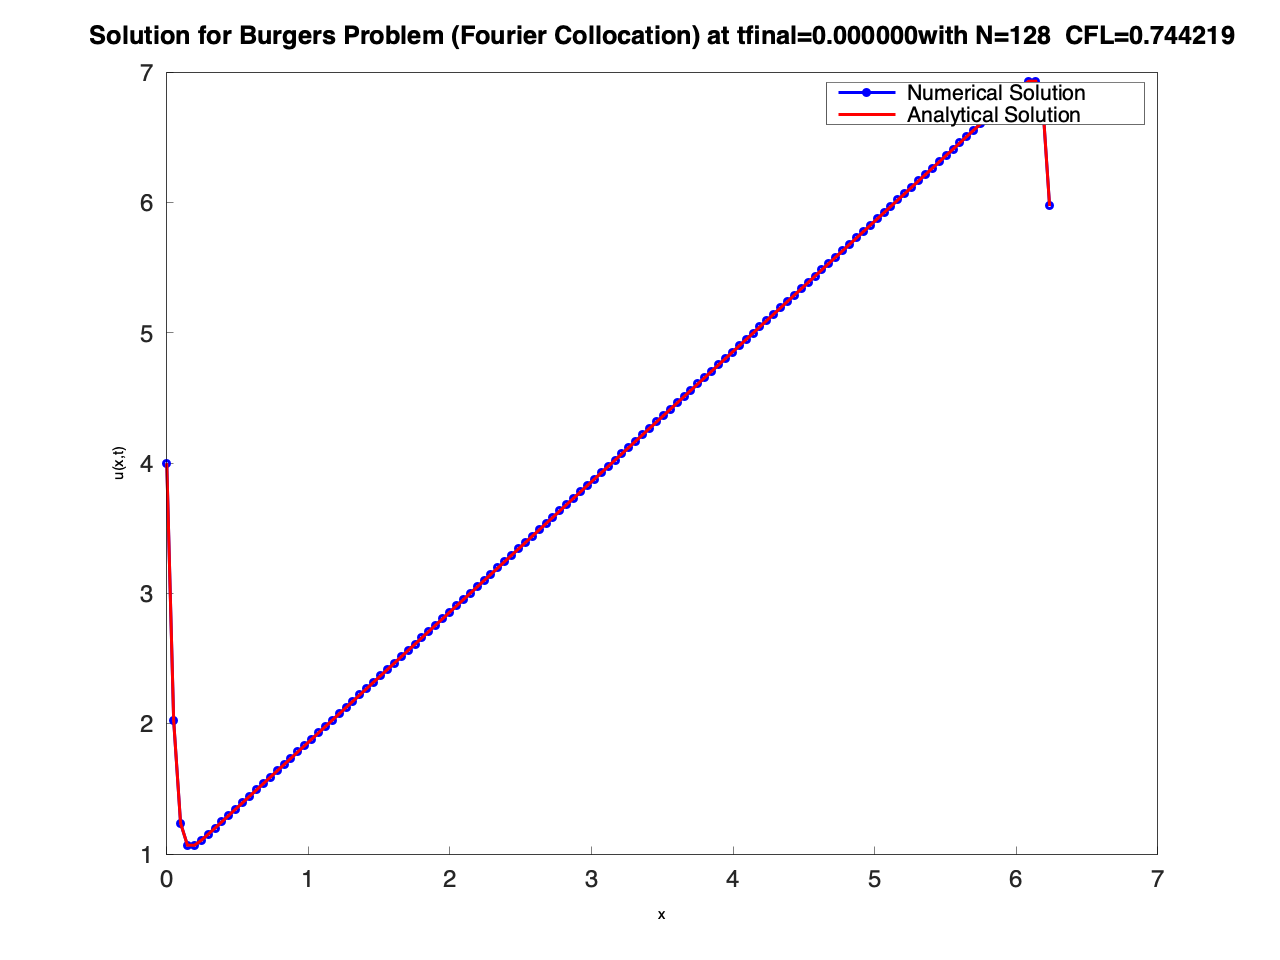
\includegraphics[width=\textwidth]{media/burger_tfinal_fc_128_0.000000.png}
		\caption{$t=0$}
		\label{sfig:sublabel1}
	\end{subfigure}%
	~
	\begin{subfigure}{0.5\textwidth}
		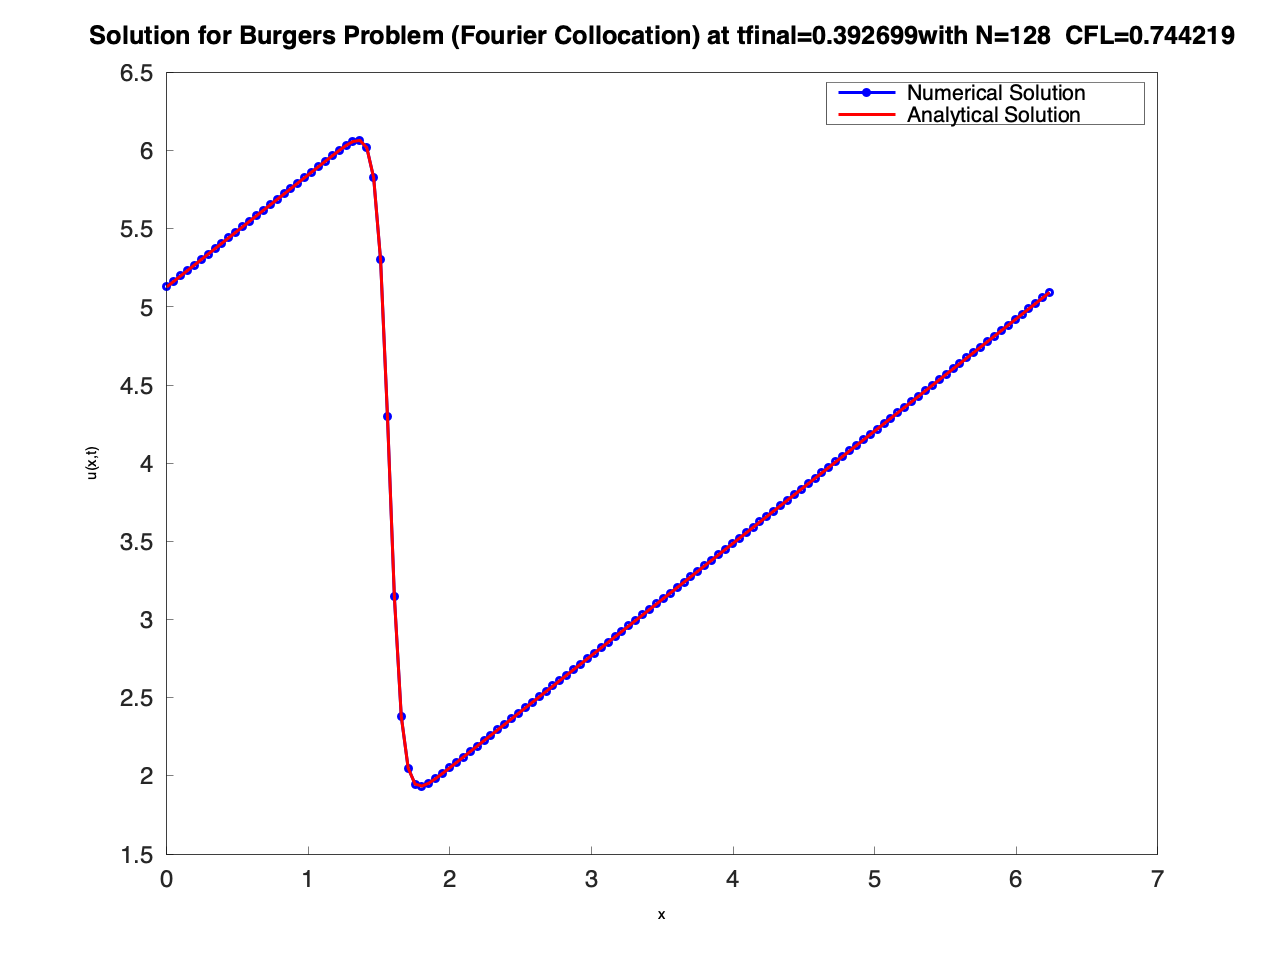
\includegraphics[width=\textwidth]{media/burger_tfinal_fc_128_0.392699.png}
		\caption{$t = \pi/ 8$}
		\label{sfig:sublabel2}
	\end{subfigure}\\
	\begin{subfigure}{0.5\textwidth}
		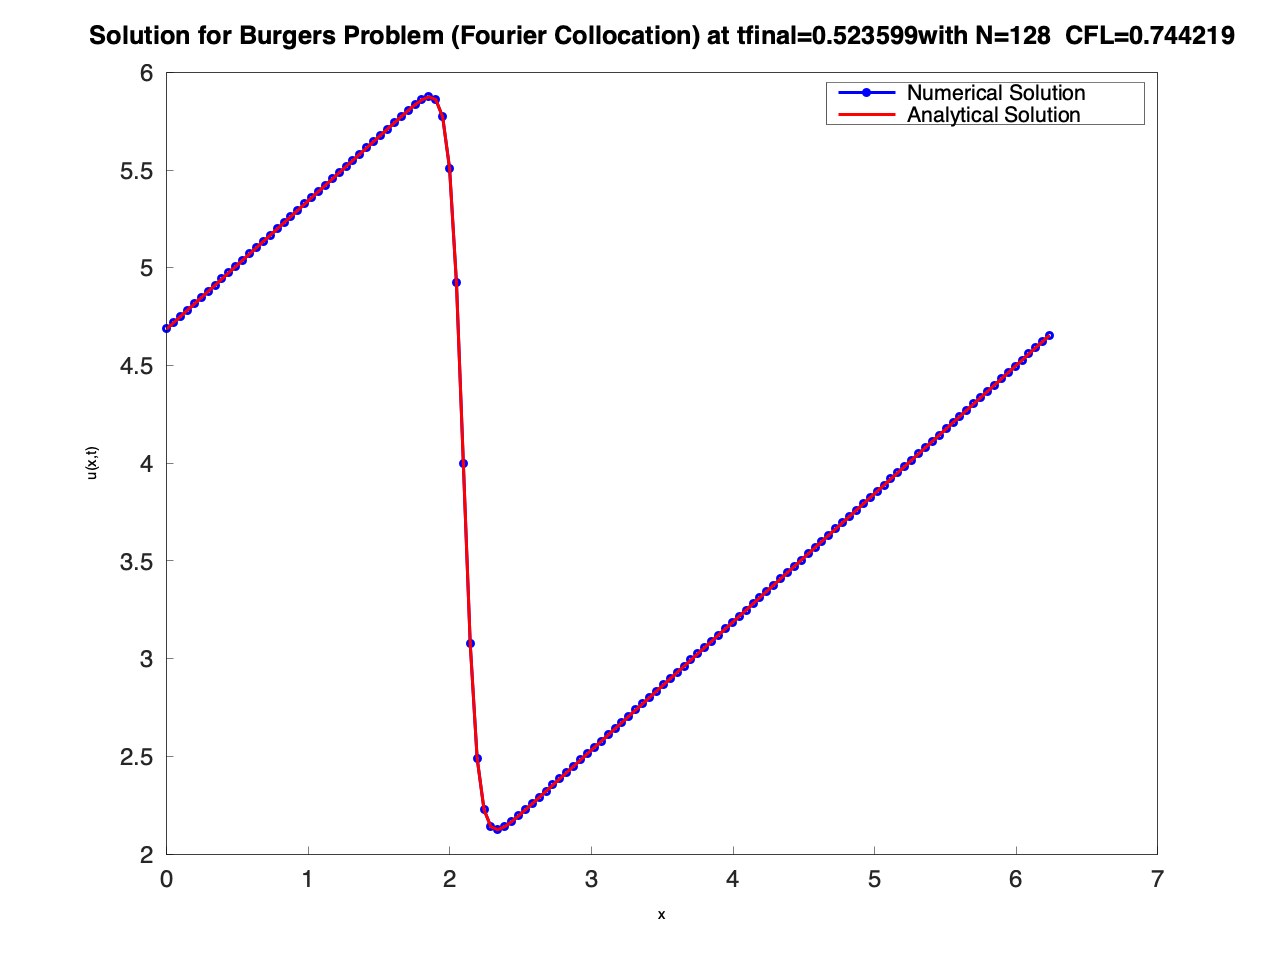
\includegraphics[width=\textwidth]{media/burger_tfinal_fc_128_0.523599.png}
		\caption{$t = \pi / 6$}
		\label{sfig:sublabel3}
	\end{subfigure}%
	~
	\begin{subfigure}{0.5\textwidth}
		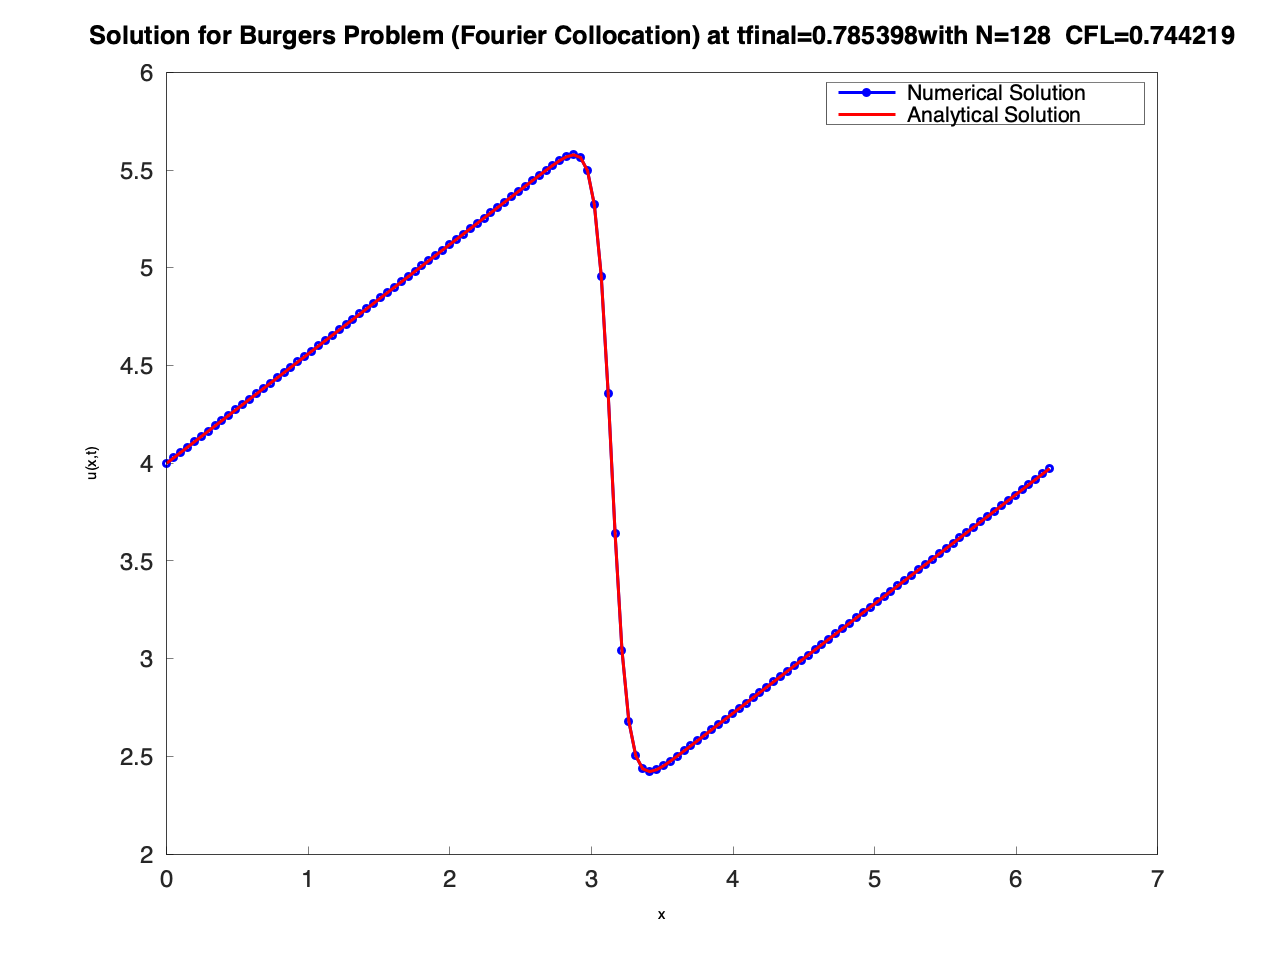
\includegraphics[width=\textwidth]{media/burger_tfinal_fc_128_0.785398.png}
		\caption{$t = \pi / 4$}
		\label{sfig:sublabel4}
	\end{subfigure}
	\caption{\textbf{Comparison of Analytical and Numerical Solution}
		The plots confirm excellent agreement between the numerical and analytical solutions at all time steps.
	}
	\label{fig:figureLabel}
\end{figure}
